
\section{Appendix}

\begin{frame}

    \label{min_wage_plot}
    
    \frametitle{State minimum wage trends} % Title
    \framesubtitle{}  % Subtitle
    \rmfamily % Font
    
    \begin{wideitemize}
        \item States have been increasing their \textcolor{fblu}{minimum wage rates}, with varying intensity
    \end{wideitemize}

    \begin{center}
        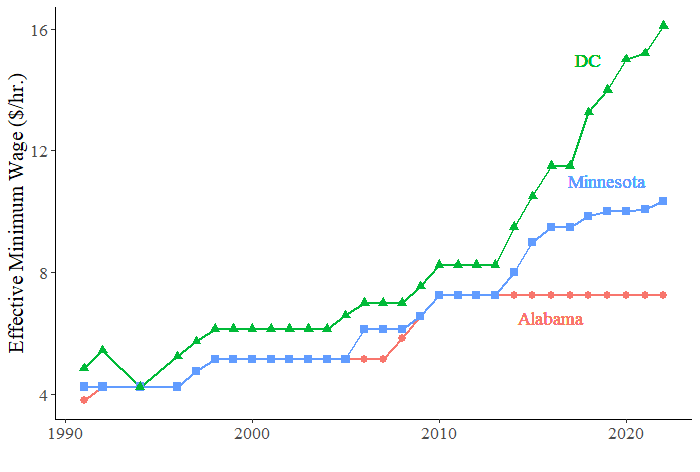
\includegraphics[scale=0.5]{min_wage_plot_simp.png}
    \end{center}
    
    \hyperlink{main_idea}{\beamerbutton{Back}}
    
\end{frame}

\begin{frame}

    \label{min_wage_plot_allstates}
    
    \frametitle{State minimum wage trends} % Title
    \framesubtitle{}  % Subtitle
    \rmfamily % Font
    
    \begin{wideitemize}
        \item States have been increasing their \textcolor{fblu}{minimum wage rates}, with varying intensity
    \end{wideitemize}

    \begin{center}
        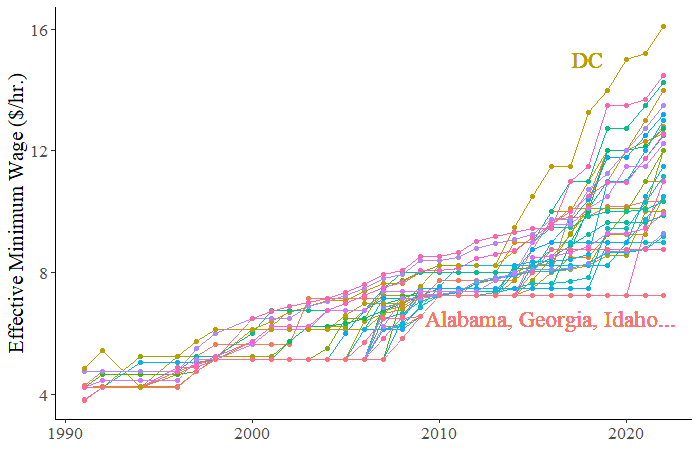
\includegraphics[scale=0.5]{min_wage_plot.png}
    \end{center}
    
    \hyperlink{main_idea}{\beamerbutton{Back}}
    
\end{frame}

\begin{frame}

    \label{quitting}
    \frametitle{Quitting decision I} % Title
    \framesubtitle{}  % Subtitle
    \rmfamily % Font

    \begin{wideitemize}
        \item Workers will quit opioids \textcolor{fblu}{if the expected utility of quitting is greater than the disutility of quitting} (\(\mathcal{C}_{quit}\))
        \item If the \textcolor{fblu}{minimum wage is not binding} and \textcolor{fblu}{the law is passed}
        \[
        q_{w_{it} > w^{min}_t} = \mathbbm{1}\{u\left(f(\theta_{it})L_{it}\right) - \mathcal{C}_{quit} \geq u\left(\left(f(\theta_{it}) - \kappa\right)L_{it}\right)\}
        \]
        \vspace{-15pt}
        \item If the \textcolor{fblu}{minimum wage is binding} and \textcolor{fblu}{the law is passed}
        \[
        q_{\,w_{it} = w^{min}_t} = \mathbbm{1}\{u\left(w^{min}_tL_{it}\right) - \mathcal{C}_{quit} \geq 0\}
        \]
    \end{wideitemize}
    
    \hyperlink{decision_making}{\beamerbutton{Back}}    

\end{frame}


\begin{frame}

    \frametitle{Quitting decision II} % Title
    \framesubtitle{}  % Subtitle
    \rmfamily % Font

    \begin{wideitemize}
        \item As long as
        \[
        u\left(f(\theta_{it})L_{it}\right) - u\left(\left(f(\theta_{it}) - \kappa\right)L_{it}\right) \geq \mathcal{C}_{quit} \geq u\left(w^{min}_tL_{it}\right)
        \]
        we should observe \textcolor{fblu}{more quitting where the minimum wage is less binding}
        \item This relation depends on \textcolor{fblu}{how much opioids affect productivity} and \textcolor{fblu}{how costly quitting is}
    \end{wideitemize}
    
    \hyperlink{decision_making}{\beamerbutton{Back}}    

\end{frame}

\begin{frame}

    \label{perc_comparison_1}
    
    \frametitle{Percentiles comparison} % Title
    \framesubtitle{}  % Subtitle
    \rmfamily % Font

    \begin{center}
        \includegraphics[scale=0.4]{mop10_unemp_rate_comp_t1.png}
    \end{center}
    
    \hyperlink{unemp_rate_result}{\beamerbutton{Back}}
    
\end{frame}

\begin{frame}

    \label{perc_comparison_12}
    
    \frametitle{Percentiles comparison} % Title
    \framesubtitle{}  % Subtitle
    \rmfamily % Font

    \begin{center}
        \includegraphics[scale=0.4]{mop10_unemp_rate_comp_t24.png}
    \end{center}
    
    \hyperlink{unemp_rate_result}{\beamerbutton{Back}}
    
\end{frame}

\begin{frame}

    \label{perc_comparison_2}
    
    \frametitle{Percentiles comparison} % Title
    \framesubtitle{}  % Subtitle
    \rmfamily % Font

    \begin{center}
        \includegraphics[scale=0.4]{mop10_emp_rate_comp_t1.png}
    \end{center}
    
    \hyperlink{emp_rate_result}{\beamerbutton{Back}}
    
\end{frame}

\begin{frame}

    \label{perc_comparison_21}
    
    \frametitle{Percentiles comparison} % Title
    \framesubtitle{}  % Subtitle
    \rmfamily % Font

    \begin{center}
        \includegraphics[scale=0.4]{mop10_emp_rate_comp_t24.png}
    \end{center}
    
    \hyperlink{emp_rate_result}{\beamerbutton{Back}}
    
\end{frame}

\begin{frame}

    \label{perc_comparison_3}
    
    \frametitle{Percentiles comparison} % Title
    \framesubtitle{}  % Subtitle
    \rmfamily % Font

    \begin{center}
        \includegraphics[scale=0.4]{mop10_lab_force_comp_t1.png}
    \end{center}
    
    \hyperlink{lab_force_rate_result}{\beamerbutton{Back}}
    
\end{frame}

\begin{frame}

    \label{perc_comparison_31}
    
    \frametitle{Percentiles comparison} % Title
    \framesubtitle{}  % Subtitle
    \rmfamily % Font

    \begin{center}
        \includegraphics[scale=0.4]{mop10_lab_force_comp_t24.png}
    \end{center}
    
    \hyperlink{lab_force_rate_result}{\beamerbutton{Back}}
    
\end{frame}

\begin{frame}

    \label{ta_1}
    
    \frametitle{Time Averages} % Title
    \framesubtitle{}  % Subtitle
    \rmfamily % Font

    \begin{center}
        \includegraphics[scale=0.4]{mop10_unemp_rate_average.png}
    \end{center}
    
    \hyperlink{unemp_rate_result}{\beamerbutton{Back}}
    
\end{frame}

\begin{frame}

    \label{ta_2}
    
    \frametitle{Time Averages} % Title
    \framesubtitle{}  % Subtitle
    \rmfamily % Font

    \begin{center}
        \includegraphics[scale=0.4]{mop10_emp_rate_average.png}
    \end{center}
    
    \hyperlink{emp_rate_result}{\beamerbutton{Back}}
    
\end{frame}

\begin{frame}

    \label{ta_3}
    
    \frametitle{Time Averages} % Title
    \framesubtitle{}  % Subtitle
    \rmfamily % Font

    \begin{center}
        \includegraphics[scale=0.4]{mop10_lab_force_average.png}
    \end{center}
    
    \hyperlink{lab_force_rate_result}{\beamerbutton{Back}}
    
\end{frame}

\begin{frame}

    \label{github_link}
    
    \frametitle{Code} % Title
    \framesubtitle{}  % Subtitle
    \rmfamily % Font
    
    \begin{center}
        \href{https://github.com/guillelozabala/masters_thesis}{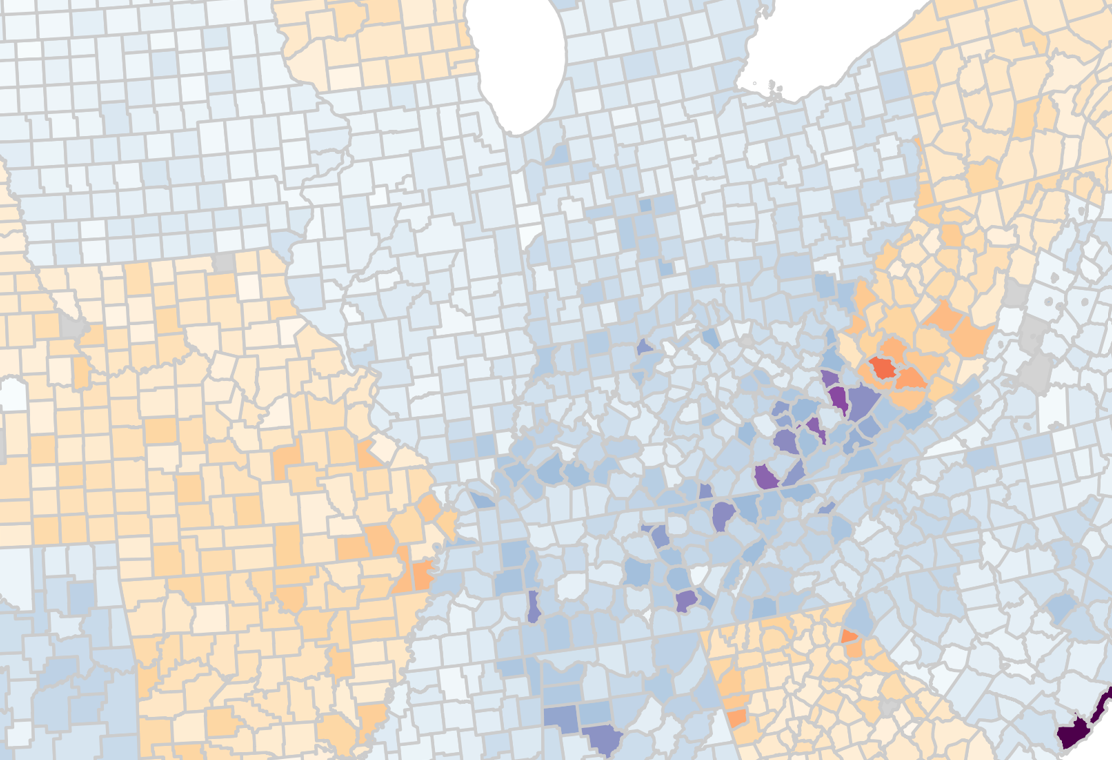
\includegraphics[scale=0.4]{thumbnail.png}}
    \end{center}
    
    %\hyperlink{}{\beamerbutton{Back}}
    
\end{frame}

